% This file was created by tikzplotlib v0.9.5.
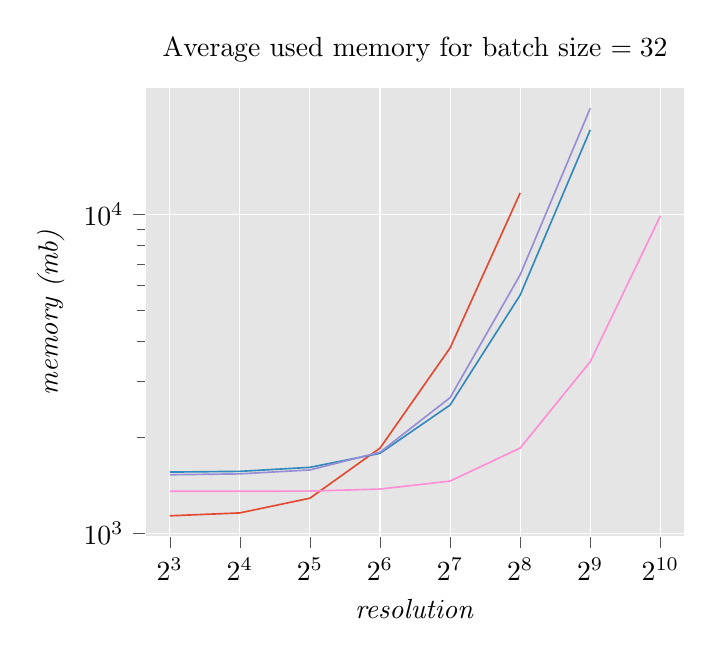
\begin{tikzpicture}

\definecolor{color0}{rgb}{0.886274509803922,0.290196078431373,0.2}
\definecolor{color1}{rgb}{0.203921568627451,0.541176470588235,0.741176470588235}
\definecolor{color2}{rgb}{0.596078431372549,0.556862745098039,0.835294117647059}
\definecolor{color3}{rgb}{0.984313725490196,0.756862745098039,0.368627450980392}
\definecolor{torchscript}{rgb}{0.996078431372549,0.556862745098039,0.835294117647059}

\begin{axis}[
axis background/.style={fill=white!89.8039215686275!black},
axis line style={white},
%legend cell align={left},
%legend style={fill opacity=0.8, draw opacity=1, text opacity=1, at={(0.03,0.97)}, anchor=north west, draw=white!80!black, fill=white!89.8039215686275!black},
log basis y={10},
tick align=outside,
tick pos=left,
title={Average used memory for batch size $=32$},
x grid style={white},
xlabel={\textit{resolution}},
xmajorgrids,
xmin=2.65, xmax=10.35,
xtick style={color=white!33.3333333333333!black},
y grid style={white},
ylabel={\textit{memory (mb)}},
ymajorgrids,
ymin=981.538600682435, ymax=24927.29576095,
ymode=log,
ytick style={color=white!33.3333333333333!black},
xticklabels={$2^3$, $2^4$, $2^5$, $2^6$, $2^7$, $2^8$, $2^9$, $2^{10}$},
xtick={3,...,10},
]
\path [fill=color0, fill opacity=0.2, very thin]
(axis cs:3,1137)
--(axis cs:3,1137)
--(axis cs:4,1161)
--(axis cs:5,1291)
--(axis cs:6,1853)
--(axis cs:7,3819)
--(axis cs:8,11683)
--(axis cs:8,11683)
--(axis cs:8,11683)
--(axis cs:7,3819)
--(axis cs:6,1853)
--(axis cs:5,1291)
--(axis cs:4,1161)
--(axis cs:3,1137)
--cycle;

\path [fill=color1, fill opacity=0.2, very thin]
(axis cs:3,1559)
--(axis cs:3,1559)
--(axis cs:4,1567)
--(axis cs:5,1613)
--(axis cs:6,1785)
--(axis cs:7,2529)
--(axis cs:8,5591)
--(axis cs:9,18415)
--(axis cs:9,18417)
--(axis cs:9,18417)
--(axis cs:8,5591)
--(axis cs:7,2529)
--(axis cs:6,1785)
--(axis cs:5,1613)
--(axis cs:4,1567)
--(axis cs:3,1559)
--cycle;

\path [fill=color2, fill opacity=0.2, very thin]
(axis cs:3,1529)
--(axis cs:3,1529)
--(axis cs:4,1539)
--(axis cs:5,1583)
--(axis cs:6,1799)
--(axis cs:7,2667)
--(axis cs:8,6473)
--(axis cs:9,21519)
--(axis cs:9,21519)
--(axis cs:9,21519)
--(axis cs:8,6473)
--(axis cs:7,2667)
--(axis cs:6,1799)
--(axis cs:5,1583)
--(axis cs:4,1539)
--(axis cs:3,1529)
--cycle;

\path [fill=white!46.6666666666667!black, fill opacity=0.2, very thin]
(axis cs:3,1357)
--(axis cs:3,1357)
--(axis cs:4,1357)
--(axis cs:5,1359)
--(axis cs:6,1379)
--(axis cs:7,1459.02)
--(axis cs:8,1849.85)
--(axis cs:9,3454.26)
--(axis cs:10,9872.04)
--(axis cs:10,9891)
--(axis cs:10,9891)
--(axis cs:9,3459)
--(axis cs:8,1855)
--(axis cs:7,1461)
--(axis cs:6,1379)
--(axis cs:5,1359)
--(axis cs:4,1357)
--(axis cs:3,1357)
--cycle;

\path [fill=torchscript, fill opacity=0.2, very thin]
(axis cs:3,1357)
--(axis cs:3,1357)
--(axis cs:4,1357)
--(axis cs:5,1359)
--(axis cs:6,1379)
--(axis cs:7,1459.02)
--(axis cs:8,1849.85)
--(axis cs:9,3454.26)
--(axis cs:10,9872.04)
--(axis cs:10,9891)
--(axis cs:10,9891)
--(axis cs:9,3459)
--(axis cs:8,1855)
--(axis cs:7,1461)
--(axis cs:6,1379)
--(axis cs:5,1359)
--(axis cs:4,1357)
--(axis cs:3,1357)
--cycle;

\addplot [semithick, color0]
table {%
3 1136.99975585938
4 1161
5 1290.99975585938
6 1853
7 3819.00048828125
8 11683.0029296875
};
%\addlegendentry{cudnn}
\addplot [semithick, color1]
table {%
3 1558.99975585938
4 1567.00024414062
5 1613.00024414062
6 1784.99975585938
7 2529.00024414062
8 5590.99951171875
9 18416.791015625
};
%\addlegendentry{libtorch}
\addplot [semithick, color2]
table {%
3 1529
4 1539.00024414062
5 1583.00036621094
6 1798.99975585938
7 2667
8 6472.998046875
9 21519.01171875
};
%\addlegendentry{pytorch}
\addplot [semithick, torchscript]
table {%
3 1356.99987792969
4 1356.99987792969
5 1359.00012207031
6 1379
7 1460.80187988281
8 1854.48486328125
9 3458.5263671875
10 9889.10546875
};
%\addlegendentry{torchscript}
\end{axis}

\end{tikzpicture}
